\chapter{Related work}

\cite{bland2022story} presents a method for breaking PDF text redaction using glyph positions; non-redacted character positioning information. In particular, subpixel-sized horizontal shifts in both the redacted and non-redacted characters can be recovered and used to effectively deredact first and last name. Breaking text-redaction schemes relies on knowing the position of characters on the page, something that is important to consider when redacting directly in a PDF instead of scanning and then OCR-ing documents. While this paper only focuses on names which may be derived from both the positioning information and potential candidates from publicly available data, this method may also be suitable for attacking other sensitive information with a reasonable length; email-addresses, phone numbers and postal addresses.
\\\\
Redaction through mosaicing and blurring where text is significantly distorted and transformed such that it is unrecognizable for the eye are popular, especially for images shared through social media. Mosaicing (pixelization) and blurring have been proven to not be viable techniques for text redaction (figure \ref{fig:blurredredaction}). Due to particular regularities in text, enough information may remain to narrow down the possibilities or even to recover the redacted text \cite{hill2016effectiveness}. A simple but powerful class of statistical models, Hidden Markov Models, can be used to recover both short and indefinitely long instances of redacted text. HMMs are used to reover sequences of characters from images of redacted text. 
\begin{figure}[h]
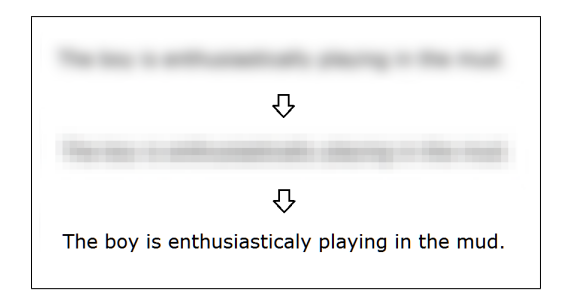
\includegraphics[width=0.7\textwidth]{latex/media/blurredRedaction.png}
\centering
\caption{Example of how a blurred image is first mosaiced, and then the text is inferred by an HMM. Not a viable option for text redaction in documents.}
\label{fig:blurredredaction}
\end{figure}
\\\\
Several methods and tools have been created to automatically find different types of redacted text in PDF documents. The X-Ray Bad Redaction Detector (X-RAY) is a fast and robust tool to identify bad redactions in PDF files \cite{Xray2021}. X-RAY detects trivial redactions where text is badly redacted under a rectangle. A technique using a combination of OCR and morphological operations has been created to detect a wide variety of different types of redaction blocks \cite{van2023detection}.
\\\\
There are several (commercially) available redaction tools which are used for text redaction and anonymization. Octobox \cite{OCTOBOX} and Zylab \cite{Zylab} are two tools frequently used by governmental bodies and municipalities in The Netherlands. \textbf{more about this}
